\documentclass[11pt]{article}
\usepackage[margin=0.75in]{geometry}
\usepackage{amsmath,amsthm,amssymb}
\usepackage{graphicx}
\usepackage{enumitem}
\usepackage{listings}
\usepackage{mathptmx}
\usepackage{comment}
\usepackage{multirow}
\usepackage{gensymb}
\lstset{
  basicstyle=\ttfamily,
  mathescape
}



\begin{document}

\title{CS 301 Lab Report 0}
\author{Sebastien James, Michael Hernandez-Thomas}
\date{\today}
\maketitle

\section*{ABSTRACT}
This lab report covers the first lab of CS 301. The lab's primary purpose is to introduce students to the actuation and sensing platforms to be used this quarter. Two simple behaviors are developed, and according measurements taken. We then discuss the result of five trials of each behavior.


\begin{comment}

Summarize the report. A good rule of thumb: 1-2 sentences on each of Sections I-IV. (Emphasis on Sections I and II.)
\end{comment}

\section*{I. INTRODUCTION}

This lab assignment is meant to serve as an introduction to the platform we will be using throughout the class. We were acquainted with the Python interface we use to gather data and perform actions on the robot, defined by Matarić as:

\begin{quote}A robot is an autonomous system which exists in the physical world, can sense its environment, and can act on it to achieve some goals.\begin{flushright}- \textit{The Robotics Primer}\end{flushright}\end{quote}

Indeed, our platform does exist in the physical world. It can gather information on its environment with a sonar, a type of sensor that uses ultrasound and echolocation to determine the distance between the sensor and any object in front of it. Other exteroceptive sensors can be used to gather information on the robot's surroundings, from buttons on a keyboard to microphones. Our platform does have a camera, but only the sonar is used in this lab. The sonar then gives a measurement which is processed into a number, corresponding to the distance between the sensor and an object. The robot also has proprioceptive sensors for each joint. The temperature and position of the servo can be fetched using thermal and positional sensors. Although not used directly, the data from the positional sensors are used whenever we want to move the robot's servo motors.

The robot platform used in the lab is a Hiwonder SpiderPi, with 18 effectors, three on each of the six legs. These effectors fulfill the next part of the definition by allowing the robot to act on its environment through movement of the whole robot. The effectors are only capable of affecting the environment through the robot's actuators. Each is a Hiwonder LX-224HV high voltage servo that is programmable in Python through a Raspberry Pi 5. This allows the robot to execute actions without human intervention, making it autonomous. The platform therefore fits Matarić's definition of a robot.

This assignment was to get the robot to perform simple actions like turning left and right, as well as designing two different behaviors for the robot. Most of the challenge did come with the confusion surrounding the version of the Raspberry Pi and software development kit. Once those problems were solved, we were able experiment with controlling the robot through the Python interface, therefore allowing future labs to cover more in-depth topics.

\begin{comment}
Introduce the topic of the lab assignment. Use terminology from the readings. Explain:
Why it is important?
What about it is challenging?
Do not yet talk about your specific approach, nor any experimental results.
Cite the readings (and any other books/papers/sites) as appropriate.
Examples of going above and beyond: Consulting references outside of the course material. Demonstrating a
particularly deep understanding or synthesis of information.
Suggested length: 1 page.

Describe/define a robot, sensors, actuators, effectors.
Identify and describe the most common types of (simple) sensing and actuation technologies, and the different layers of
sensor processing.
\end{comment}



\section*{II. METHODS}

The lab can be divided into two sub-tasks: discovering how the robot works and figuring out hexapod locomotion. 

After looking through the code for the sonar, it seems to request two bytes of data from the bus. It then converts those bytes into an integer between 0 and 5000, with lower numbers corresponding to lower distances to the object. This is all wrapped in the \lstinline{getDistance} function in the \lstinline{sonar.py} file provided to us. We therefore can interpret the value given to us as the distance from the sonar to the obstacle.

The servos for the legs are numbered from 1 to 18, with the numbers starting at the back of the robot at the closest servo to the body, then extending outward and forwards. The IDs then cycle towards the front of the robot on the left side of the body before repeating on the right. Each servo can be set programmatically to a position in the range 0 to 1000. To make the servo IDs clearer to us, we grouped them based on their approximate function if mapped to the human body: the closest to the body (1, 4, 7, 10, 13, 16) are the \lstinline{hips}, the second from the body (2, 5, 8, 11, 14, 17) are the \lstinline{knees}, and the last group (3, 6, 9, 12, 15, 18) are the \lstinline{ankles}.

\begin{figure}[h]
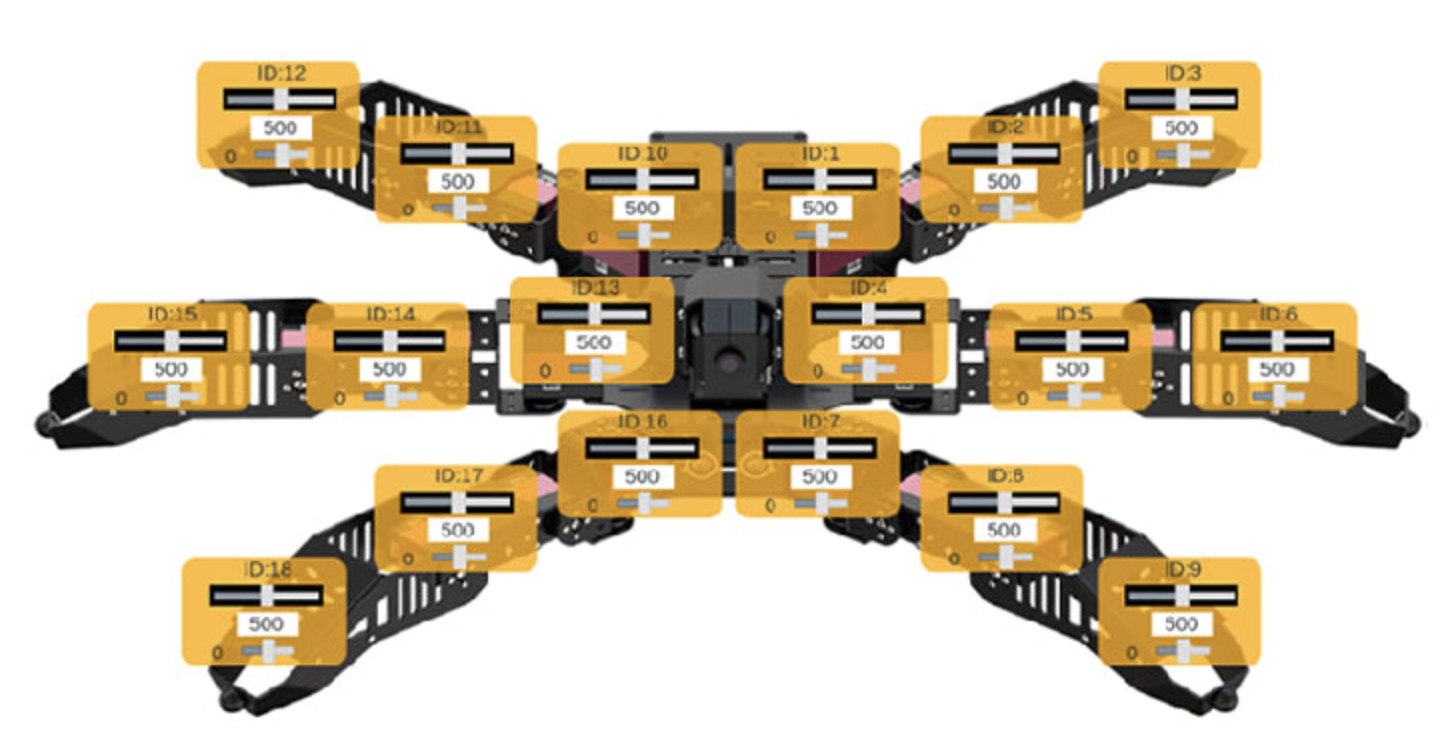
\includegraphics[width=160mm]{ids.png}
\centering
\end{figure}


Our first challenge was to figure out how to turn the robot. Our approach involved lifting all the legs, leaving the chassis of the robot on the floor, rotating the legs, setting them back down, lifting the body back up, and finally returning to the original position. Doing this lets the robot turn up to 45 degrees to either side, using the available range of motion of the legs. 

The more complicated challenge involved designing and implementing two behaviors for the robot. After making the robot turn, naturally we wanted to make the robot move forwards. Initially we tried reusing our idea for turning the robot, but that would involve dragging the metal body of the robot on the floor. Out of concern for both the robot and the floor's safety, we instead looked to move the legs in two groups of three to keep the robot "standing" while moving. To add sensors to this behavior, we made the robot walk forward until it detects an obstacle in front of it.

Our second behavior makes the robot scan in the four cardinal directions, and turn towards the direction with the smallest distance to an obstacle. This is achieved by using the turning script we developed previously. After turning 90 degrees, the robot reads from the sonar and stores that value. Once all four scans are saved, the robot then compares the distances and turns towards the direction with the smallest value.


To assess the accuracy of our behaviors, we ran five repetitions of the same test. For the first behavior, the test started with the robot at 1 meter from the wall (measured from the sonar). The robot then walked forward until within 300 units of distance measured by the sonar. The distance from the wall and deviation from the center line were recorded to measure the preciseness of the robot's behavior. This allows us to see if our behavior is capable of walking straight, as well see if it stops at a consistent distance from the wall.
The second behavior was assessed by measuring the error in degrees of the full rotation, and recording the shortest distance measured by the sonar. These measurements will allow us to precisely tune how much the hip joints need to rotate to achieve a 90 degree turn.


\begin{comment}

Describe in detail your approach to solving the lab's challenge. Include a thorough description of any developed processing/algorithms, that covers:
The sensor input, and sensor processing.
The algorithm reasoning.
The actuation output.
(This description should be at a conceptual level, and should not describe the low-level details of your code.)
Provide a clear and convincing motivation for your approach.
Cite the readings (and any other books/papers/sites) as appropriate.
Clearly describe the experimental tests you will run to empirically validate your approach.
Explain why these tests were chosen. (What will the tests show?)
Examples of going above and beyond: An algorithm or hardware design that is particularly clever, or more complex to implement.
Suggested length: 1-2 pages.

Describe all of the sensors and actuators on the robot platform your group has decided to build – how they work, what they are used for. Use terminology from the readings.
Provide a description of your implementation of step B-5.
Be sure to clearly describe your planned experimental work (i.e., planned measurements)

\end{comment}

\section*{III. RESULTS}



From our first test, the robot was placed 1 meter from the wall, centered over a line in the tiles. This allowed us to measure the stopping distance from the wall and the deviation from the center line. The distance from the wall was measured from the front of the sonar to the wall, and the deviation was measured from the line on the tiles to the center of the robot.
\begin{figure}[h!]
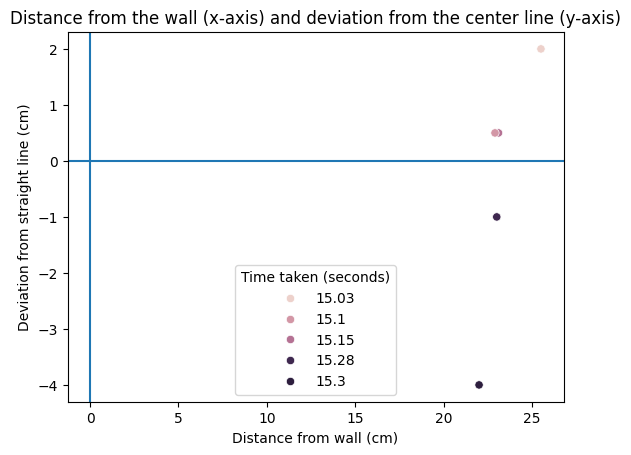
\includegraphics[width=120mm]{behavior1.png}
\centering
\end{figure}

$\sigma_{wall} = 1.166 $cm$, \sigma_{center} = 2.035 $cm$, \sigma_{time} = 0.104 $s


$m_{wall} = 23.3 $cm$, m_{center} = -0.4 $cm$, m_{time} = 15.172 $s



Our second test involved setting the robot on the floor with an obstacle on one of its cardinal directions. We attached a phone compass on top to set the angle to 29 degrees at the start of the test. We then let the behavior perform, and at the end measured whether it turned to the right direction. Additionally, we printed out the minimum value the sonar read and recorded it. Trials 1 through 3 had the obstacle in front of the starting position, while trial 4 had the obstacle behind the robot, and 5 had the obstacle to the right of the robot.\\


\begin{tabular}{ |p{3cm}||p{4cm}|p{5cm}|p{3cm}|  }
 \hline
 \multicolumn{4}{|c|}{Behavior 2 Measurement Results} \\
 \hline
 Trial number & Turn Error (degrees) & Distance to Closest Obtacle (cm) & Right direction?\\
 \hline
 1 & 10 &256&   Yes\\
 2 &  10  & 261   &Yes\\
 3 &10 & 277&  Yes\\
 4 &15 & 405&  Yes\\
 5 (compass started at 337) & 50 & 392&Yes\\
 \hline
\end{tabular}\\

$\sigma_{obstacle\_distance} = 66.059 $cm$, \sigma_{turn\_error} =  2.332 \degree$

$m_{obstacle\_distance} = 318.2 $cm$, m_{turn\_error} =  29.6 \degree$

\begin{comment}

Report the data collected and analyzed from your experimental testing.
Make sure to label all axes, define variables/parameters, give units for all variables, title plots.
Clearly describe the details of your experimental conditions and data collection techniques.
(Under what conditions was a measurement performed, and using what measurement tool?)
Include statistics, figures and tables, as appropriate.
The presentation of your data should be concise and thorough. For example, displaying multiple experimental conditions on the same plot is often easier for the reader to digest, and as a bonus also takes up less space.
Examples of going above and beyond: Gathering an extra type of experimental data.
Suggested length: 1-2 pages.

Perform each of your chosen measurements a minimum of 5 times.
Report averages, with standard deviations.
Be sure to clearly describe all data collection procedures and testing conditions.

\end{comment}

\section*{IV. DISCUSSION}

\subsection*{Behavior 1}

We can see that the robot is consistent in its stopping distance and time taken to arrive at the wall. However, it seems to deviate somewhat in its path. This is probably explained by how the robot was set up in the test. It was lined up on the ground in a top-down fashion, letting it be precisely aligned at the 1 meter mark. However, it was harder to align it to be perfectly straight, causing the perceived deviation from the center line. A different method of setting up the robot, like having markers for the location of the feet, would allow for more precise alignment.

The timing of the robot arriving in roughly 15 seconds is also expected, as the walk cycle takes 1 second per cycle. The extra decimals can be accounted for the delay is us stopping the timer.

\subsection*{Behavior 2}

The turn error was very consistent, except for one trial run. This could be explained by a consistent understeer that accumulates the more the robot needs to turn. Since the robot makes left turns, it needs to turn less times for the obstacle on the left. The error was precise enough each time that after four turns, the robot was always 10\degree off. This is further supported by the error after 6 turns being 15\degree off, leading us to believe that each 90\degree  turn was actually a 87.5\degree  turn.

The last trial can be discarded. We found out that the phone compass is really inaccurate, giving different readings when clearing facing the same direction. Tilting the vertically seemed to make the compass lose its position. As such, the trial should probably be redone with a different measuring instrument, like a protractor.

\begin{figure}[h!]
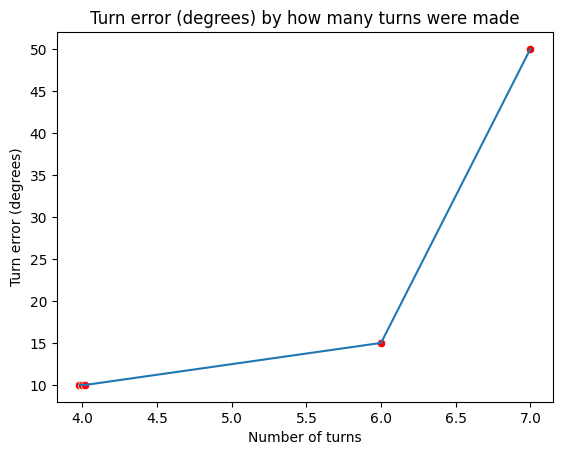
\includegraphics[width=120mm]{behavior2c.png}
\centering
\end{figure}

\begin{comment}
Provide a discussion of your observed results, and any insights you have gained about the lab topic.
Don't just repeat the data reported in the RESULTS section, but rather provide a higher-level analysis of your observed results.
What were the positive results?
Are there any key aspects of your approach that accounted for them?
Where is there room for improvement: with respect to the empirical results, data collection, algorithm, etc?
How do your results change/support the way you look at the lab topic (with respect to its perceived challenges,
importance within the field, etc.)?
Examples of going above and beyond: Demonstrating particularly deep insight or observations.
Suggested length: 1-2 pages

Discuss the performance of each of your developed behaviors.
How accurate do you expect each of your measurements are, and why?
What are some potential sources of noise and/or uncertainty?

\end{comment}
\section*{V. CONCULSION}
The behaviors developed explore the use of both the actuators and sensor of our platform. We developed an introductory turning behavior, a walk until in front of a wall behavior, and a turn towards the closest object behavior. One behavior works as intended, while the other could use some improvement in both implementation and measurements.

\begin{comment}
Recap the report. A good rule of thumb: 1-3 sentences to each of Sections II-IV. (Emphasis on Sections III and IV.
\end{comment}

\section*{REFERENCES}

Matarić, M. J. (2008). The Robotics Primer. The MIT Press. 

\end{document}